\documentclass[tikz, preview]{standalone}

\usepackage{amsfonts, amsthm, amssymb, amsmath, stmaryrd, etoolbox}
\usepackage{tikz}
\usepackage[all,2cell]{xy}
\usetikzlibrary{matrix,arrows,shapes,decorations.markings,decorations.pathreplacing}
\definecolor{rewritecolor}{rgb}{0,.9,1}
\tikzset{rewritenode/.style={shape=circle,fill=rewritecolor,scale=0.25,font=\Huge}}
\tikzset{RWopen/.style={shape=circle,draw=black,fill=white,scale=0.5,font=\Huge}}
\tikzset{RWclosed/.style={shape=circle,fill=black,scale=0.5,font=\Huge}}
\tikzset{CDnode/.style={shape=circle,fill=white,scale=.5}}
\tikzset{zxgreen/.style={shape=circle,draw,thick,fill=green}}
\tikzset{zxred/.style={shape=circle,draw,thick,fill=red}}
\tikzset{zxyellow/.style={shape=rectangle,draw,thick,fill=yellow}}
\tikzset{zxdiamond/.style={shape=diamond,fill=black,inner sep=2.75}}
\tikzset{zxopen/.style={shape=circle,draw,thick,inner sep=2pt}}
\tikzset{->-/.style={decoration={markings,mark=at position .5 with {\arrow{>}}},postaction={decorate}}}
\tikzset{->-pos/.style={decoration={
			markings,
			mark=at position #1 with {\arrow{>}}},postaction={decorate}}}


\begin{document}
\[
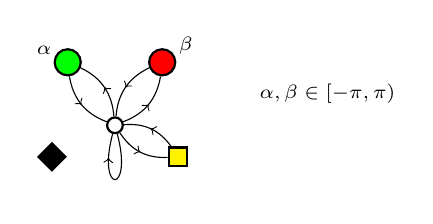
\begin{tikzpicture}
\node [zxopen] (v1) at (0,0) {};
\node [zxgreen,label={[shift={(-.3,-.2)}]\scriptsize $\alpha$}] (v2) at (-0.6,0.8) {};
\node [zxyellow] (v3) at (0.8,-0.4) {};
\node [zxdiamond] (v5) at (-0.8,-0.4) {};
\node [zxred,label={[shift={(.3,-.2)}]\scriptsize $\beta$}] (v4) at (0.6,0.8) {};
\node at (2.7,0.4) {\scriptsize $\alpha, \beta \in [-\pi,\pi)$};
%
\draw [->-] (v1) to [bend right] (v2);
\draw [->-] (v2) to [bend right] (v1);
\draw [->-] (v1) to [bend right] (v3);
\draw [->-] (v3) to [bend right] (v1);
\draw [->-] (v1) to [bend right] (v4);
\draw [->-] (v4) to [bend right] (v1);
\draw [->-pos=0.75]  (v1) to [loop below, looseness=35] (v1);
\end{tikzpicture}
\]
\end{document}
